\documentclass[12pt,a4paper]{article}
\usepackage[utf8]{vietnam}
\usepackage{amsmath,amssymb,amsfonts}
\usepackage[left=1.5cm,right=1.5cm,top=2cm,bottom=2cm,headheight=17pt]{geometry}
\usepackage{enumitem,array,graphicx,tikz,fancyhdr,needspace}
\usetikzlibrary{arrows.meta,calc,patterns}
\pagestyle{fancy}
\fancyhf{}
\lhead{\small\textbf{HƯỚNG TỚI THPTQG 2027}}
\rhead{\small\textit{Người biên soạn: Dương Gia Bảo}}
\rfoot{\small Trang \thepage}
\renewcommand{\headrulewidth}{0.4pt}
\setlength{\parindent}{0pt}
\setlength{\parskip}{3pt}
\setlist[enumerate,1]{label=\textbf{Câu \arabic*:},leftmargin=*,itemsep=9pt,topsep=6pt}
\setlist[enumerate,2]{label=\alph*),leftmargin=*,itemsep=3pt,topsep=4pt}
\newcommand{\bonpa}[4]{\par\smallskip\noindent
  \begin{tabular}{@{}p{0.47\linewidth}p{0.47\linewidth}@{}}
  \textbf{A.} #1 & \textbf{B.} #2\\[3pt]
  \textbf{C.} #3 & \textbf{D.} #4
  \end{tabular}}
\newcommand{\loigiai}[1]{\par\medskip\Needspace{4\baselineskip}\noindent\textbf{#1}\par\nobreak}
\begin{document}
\noindent
\begin{minipage}[t]{0.40\textwidth}
    \centering
    \textbf{HƯỚNG TỚI THPTQG 2027}\\[-2pt]
    \rule{3.2cm}{0.6pt}\\[4pt]
    \textbf{ĐỀ CHÍNH THỨC}
\end{minipage}\hfill
\begin{minipage}[t]{0.58\textwidth}
    \centering
    \textbf{ĐỀ THI KHẢO SÁT CHẤT LƯỢNG}\\
    \textbf{ĐỀ SỐ 12}\\
    \textbf{Môn thi: TOÁN}\\
    \textit{\small Thời gian làm bài: 90 phút, không kể thời gian phát đề}
\end{minipage}
\vspace{0.2cm}
\noindent
\begin{minipage}[b]{0.78\textwidth}
    \textbf{Họ và tên:}\dotfill\textbf{SBD:}\makebox[3.5cm]{\dotfill}
\end{minipage}\hfill
\begin{minipage}[b]{0.20\textwidth}
    \hfill\setlength{\fboxrule}{0.8pt}
    \fbox{\begin{minipage}{2.3cm}\centering
      \textbf{\small Mã đề thi}\\\textbf{0012}
    \end{minipage}}
\end{minipage}
\vspace{0.2cm}

\section*{\large PHẦN I. CÂU TRẮC NGHIỆM NHIỀU PHƯƠNG ÁN LỰA CHỌN}
\textit{Thí sinh trả lời từ câu 1 đến câu 12. Mỗi câu chỉ chọn một phương án. Mỗi câu trả lời đúng được 0,25 điểm.}
\begin{enumerate}
\item Cho hàm số $y=\dfrac{x^2-2x+5}{x-1}$. Hàm số đồng biến trên khoảng nào sau đây?
\bonpa{$(-1;1)$.}{$(3;+\infty)$.}{$(1;3)$.}{$(-1;3)$.}

\item Nghiệm của phương trình $\log_2(x-1)+\log_2(x+1)=3$ là
\bonpa{$x=-3$.}{$x=\sqrt{7}$.}{$x=2$.}{$x=3$.}

\item Giá trị của tích phân $\displaystyle\int_0^2(3x^2-2x+1)\,\mathrm{d}x$ bằng
\bonpa{$6$.}{$8$.}{$4$.}{$10$.}

\item Trong không gian $Oxyz$, mặt phẳng qua $M(2;-1;3)$ và vuông góc với đường thẳng có vectơ chỉ phương $\vec u=(1;2;-1)$ có phương trình là
\bonpa{$x+2y-z-3=0$.}{$x-2y+z-7=0$.}{$x+2y-z+3=0$.}{$2x+y-z=0$.}

\item Một hộp có $5$ viên bi đỏ và $3$ viên bi xanh, các viên bi cùng kích thước và khối lượng. Lấy ngẫu nhiên đồng thời $2$ viên bi. Xác suất để cả hai viên đều đỏ bằng
\bonpa{$\dfrac{25}{64}$.}{$\dfrac{5}{8}$.}{$\dfrac{3}{14}$.}{$\dfrac{5}{14}$.}

\item Thời gian hoàn thành một tác vụ (phút) của $30$ người được thống kê như sau:
\begin{center}
\begin{tabular}{|c|c|c|c|c|}\hline
Thời gian & $[0;10)$ & $[10;20)$ & $[20;30)$ & $[30;40)$\\\hline
Số người & $4$ & $8$ & $12$ & $6$\\\hline
\end{tabular}
\end{center}
Trung vị của mẫu số liệu ghép nhóm này bằng
\bonpa{$20$.}{$22{,}5$.}{$25$.}{$27{,}5$.}

\item Tập nghiệm của phương trình $2\sin x=1$ trên khoảng $[0;2\pi)$ là
\bonpa{$\left\{\dfrac{\pi}{6};\dfrac{5\pi}{6}\right\}$.}{$\left\{\dfrac{\pi}{6};\dfrac{7\pi}{6}\right\}$.}{$\left\{\dfrac{\pi}{3};\dfrac{2\pi}{3}\right\}$.}{$\left\{\dfrac{5\pi}{6};\dfrac{11\pi}{6}\right\}$.}

\item Cho cấp số nhân $(u_n)$ có $u_1=2$ và công bội $q=3$. Giá trị $u_5$ bằng
\bonpa{$54$.}{$486$.}{$162$.}{$48$.}

\item Trong không gian $Oxyz$, mặt cầu có tâm $I(1;-1;2)$ và tiếp xúc với mặt phẳng $(P):2x-y+2z+2=0$. Bán kính mặt cầu bằng
\bonpa{$3$.}{$1$.}{$9$.}{$\sqrt{3}$.}

\item Cho hàm số $f(x)=x+1+\dfrac{4}{x-2}$. Có bao nhiêu giá trị nguyên $m$ thuộc đoạn $[-3;10]$ để phương trình $f(x)=m$ có hai nghiệm thực phân biệt?
\bonpa{$4$.}{$6$.}{$7$.}{$5$.}

\item Một đèn tròn bán kính $0{,}6\,\mathrm m$, trọng lượng $90\,\mathrm N$ được treo nằm ngang bằng ba dây không dãn có cùng độ dài $L$. Một đầu mỗi dây buộc vào cùng một điểm trên trần, nằm trên đường thẳng đứng qua tâm đèn; các đầu còn lại buộc vào ba điểm chia đều vành đèn. Mỗi dây chịu được lực căng tối đa $50\,\mathrm N$. Bỏ qua khối lượng dây. Độ dài nhỏ nhất của mỗi dây là
\bonpa{$0{,}60\,\mathrm m$.}{$0{,}75\,\mathrm m$.}{$0{,}80\,\mathrm m$.}{$1{,}00\,\mathrm m$.}

\item Hộp $A$ chứa $4$ viên bi đỏ và $2$ viên bi xanh; hộp $B$ chứa $2$ viên bi đỏ và $4$ viên bi xanh. Các viên bi cùng kích thước và khối lượng. Chọn ngẫu nhiên một hộp, hai hộp có xác suất được chọn bằng nhau, rồi lấy ngẫu nhiên đồng thời $2$ viên bi từ hộp đó. Biết cả hai viên lấy ra đều đỏ, xác suất hộp đã chọn là hộp $A$ bằng
\bonpa{$\dfrac{2}{3}$.}{$\dfrac{4}{5}$.}{$\dfrac{6}{7}$.}{$\dfrac{1}{2}$.}
\end{enumerate}

\Needspace{18\baselineskip}
\section*{\large PHẦN II. CÂU TRẮC NGHIỆM ĐÚNG SAI}
\textit{Thí sinh trả lời từ câu 1 đến câu 4. Trong mỗi ý a), b), c), d), chọn đúng hoặc sai. Ở mỗi câu, chọn chính xác 1, 2, 3, 4 ý lần lượt được 0,1; 0,25; 0,5; 1 điểm.}
\begin{enumerate}
\item \begin{minipage}[t]{0.55\linewidth}
Cho hàm số $f(x)=\dfrac{x^2-4x+8}{x-2}$ có đồ thị $(C)$ như hình bên. Gọi $I$ là giao điểm hai đường tiệm cận của $(C)$.
\begin{enumerate}[label=\alph*)]
\item Đường tiệm cận xiên của $(C)$ là $y=x+2$.
\item Khoảng cách giữa hai điểm cực trị của $(C)$ bằng $4\sqrt{5}$.
\item Tiếp tuyến tại điểm có hoành độ $x=3$ cắt hai đường tiệm cận tại $A$, $B$. Diện tích tam giác $IAB$ bằng $8$.
\item Có đúng $3$ giá trị nguyên $m$ để phương trình $f(x)=m$ có hai nghiệm phân biệt $x_1,x_2$ thỏa mãn $2<x_1<x_2<8$.
\end{enumerate}
\end{minipage}\hfill
\begin{minipage}[t]{0.42\linewidth}
\vspace{-0.4\baselineskip}\centering
\resizebox{\linewidth}{!}{%
\begin{tikzpicture}[>=Stealth,line cap=round,line join=round,x=0.8cm,y=0.40cm,font=\large]
\draw[->] (-3,0)--(7.5,0) node[right] {$x$};
\draw[->] (0,-9)--(0,9.5) node[above] {$y$};
\draw[dashed,gray] (2,-9)--(2,9);
\draw[dashed,gray] (-3,-5)--(7,5);
\draw[blue!55!black,very thick,domain=-3:1.5,samples=100] plot (\x,{\x-2+4/(\x-2)});
\draw[blue!55!black,very thick,domain=2.5:7,samples=100] plot (\x,{\x-2+4/(\x-2)});
\draw[densely dotted] (0,4)--(4,4)--(4,0);
\fill (0,-4) circle (2pt);\fill (4,4) circle (2pt);\fill (2,0) circle (2pt);
\node[below left,fill=white,inner sep=1pt] at (0,0) {$O$};
\node[above left,fill=white,inner sep=1pt] at (2,0) {$I$};
\node[below,fill=white,inner sep=1pt] at (2,0) {$2$};
\node[below] at (4,0) {$4$};
\node[left,fill=white,inner sep=1pt] at (0,4) {$4$};
\node[left,fill=white,inner sep=1pt] at (0,-4) {$-4$};
\end{tikzpicture}}
\end{minipage}

\item Một nhà máy có hai phân xưởng $A$, $B$ sản xuất lần lượt $40\%$, $60\%$ tổng số linh kiện. Tỉ lệ linh kiện lỗi của hai phân xưởng lần lượt là $2\%$, $5\%$. Chọn ngẫu nhiên một linh kiện từ toàn bộ sản phẩm. Linh kiện được kiểm tra hai lần bằng cùng một quy trình: mỗi lần, xác suất báo lỗi là $0{,}9$ nếu linh kiện thực sự lỗi và là $0{,}1$ nếu linh kiện không lỗi. Giả sử hai kết quả kiểm tra độc lập khi đã biết trạng thái lỗi hay không lỗi của linh kiện, và quy trình không phụ thuộc phân xưởng sản xuất.
\begin{enumerate}[label=\alph*)]
\item Xác suất linh kiện được chọn thực sự lỗi bằng $0{,}038$.
\item Biết linh kiện thực sự lỗi, xác suất nó do phân xưởng $A$ sản xuất bằng $\dfrac{6}{19}$.
\item Xác suất cả hai lần kiểm tra đều báo lỗi bằng $0{,}0344$.
\item Biết cả hai lần kiểm tra đều báo lỗi, xác suất linh kiện thực sự lỗi lớn hơn $75\%$.
\end{enumerate}

\item \begin{minipage}[t]{0.55\linewidth}
Trong không gian $Oxyz$ (đơn vị: km), radar đặt tại $O$ phát hiện được drone khi khoảng cách đến drone không vượt quá $5$ km. Drone chuyển động thẳng đều; tại thời điểm $t$ phút ($t\geq0$), vị trí của nó là $M(-7+2t;-10+2t;-2+t)$. Hình bên minh họa trong mặt phẳng chứa $O$ và đường bay $d$; $A$ là vị trí ban đầu.
\begin{enumerate}[label=\alph*)]
\item Khoảng cách từ $O$ đến vị trí ban đầu của drone bằng $3\sqrt{17}$ km.
\item Drone gần radar nhất tại thời điểm $t=4$ phút.
\item Tổng thời gian drone nằm trong vùng phát hiện của radar bằng $3$ phút.
\item Để thời gian phát hiện drone ít nhất $4$ phút, bán kính vùng phát hiện chỉ cần đạt từ $6$ km trở lên.
\end{enumerate}
\end{minipage}\hfill
\begin{minipage}[t]{0.42\linewidth}
\vspace{-0.4\baselineskip}\centering
\resizebox{\linewidth}{!}{%
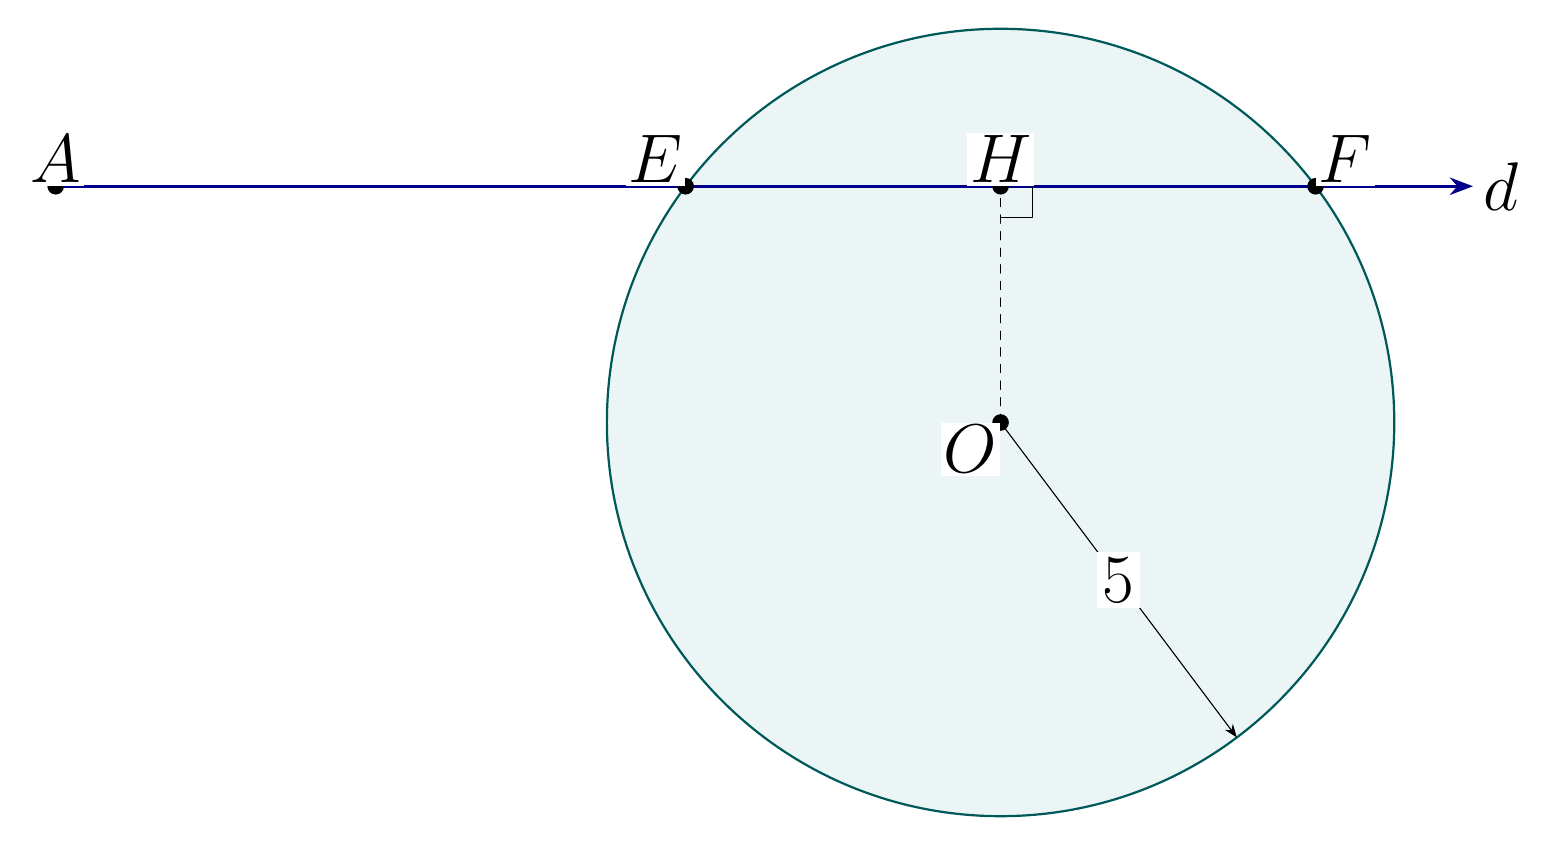
\begin{tikzpicture}[>=Stealth,line cap=round,line join=round,font=\Huge]
\fill[teal!8] (0,0) circle (5);
\draw[teal!70!black,thick] (0,0) circle (5);
\draw[->,blue!55!black,very thick] (-12,3)--(6,3) node[right,black] {$d$};
\draw[dashed] (0,0)--(0,3);
\draw (0,2.6)--(0.4,2.6)--(0.4,3);
\draw[->] (0,0)--(3,-4) node[midway,fill=white,inner sep=2pt] {$5$};
\fill (0,0) circle (3pt) node[below left,fill=white,inner sep=1pt] {$O$};
\fill (0,3) circle (3pt) node[above,fill=white,inner sep=1pt] {$H$};
\fill (-12,3) circle (3pt) node[above,fill=white,inner sep=1pt] {$A$};
\fill (-4,3) circle (3pt) node[above left,fill=white,inner sep=1pt] {$E$};
\fill (4,3) circle (3pt) node[above right,fill=white,inner sep=1pt] {$F$};
\end{tikzpicture}}
\end{minipage}

\item Một máy đóng gói được kiểm tra bằng cách cân $50$ gói hàng. Khối lượng (gam) được thống kê thành mẫu số liệu ghép nhóm sau:
\begin{center}
\begin{tabular}{|c|c|c|c|c|c|}\hline
Khối lượng & $[48;50)$ & $[50;52)$ & $[52;54)$ & $[54;56)$ & $[56;58)$\\\hline
Số gói & $5$ & $10$ & $20$ & $10$ & $5$\\\hline
\end{tabular}
\end{center}
Các số đo dưới đây được tính theo mẫu số liệu ghép nhóm.
\begin{enumerate}[label=\alph*)]
\item Khối lượng trung bình bằng $53$ gam.
\item Phương sai bằng $4{,}6$ gam$^2$.
\item Khoảng tứ phân vị bằng $3$ gam.
\item Nếu máy được hiệu chỉnh để mỗi giá trị khối lượng $X$ chuyển thành $Y=0{,}5X+26{,}5$, khối lượng trung bình không đổi và độ lệch chuẩn giảm còn một nửa.
\end{enumerate}
\end{enumerate}

\Needspace{8\baselineskip}
\section*{\large PHẦN III. CÂU TRẮC NGHIỆM TRẢ LỜI NGẮN}
\textit{Thí sinh trả lời từ câu 1 đến câu 6. Mỗi câu trả lời đúng được 0,5 điểm. Chỉ làm tròn ở kết quả cuối cùng.}
\begin{enumerate}
\item Một hãng bán tai nghe có giá bán mỗi chiếc là $800$ nghìn đồng và chi phí sản xuất mỗi chiếc là $500$ nghìn đồng. Nếu chi $x$ triệu đồng cho quảng cáo ($x\geq0$), số tai nghe bán được theo mô hình là $n(x)=A+40\ln(1+x)$, trong đó $A$ là hằng số. Biết khi chi $e^2-1$ triệu đồng cho quảng cáo, số tai nghe bán được theo mô hình là $200$ chiếc. Giả sử bán hết số tai nghe sản xuất, không có chi phí khác và sử dụng trực tiếp số lượng thực $n(x)$ trong mô hình. Lợi nhuận lớn nhất của hãng bằng bao nhiêu triệu đồng? \textit{(Làm tròn đến hàng phần mười.)}

\item \begin{minipage}[t]{0.55\linewidth}
Một bể nước có chiều rộng không đổi $6$ m, sâu $3$ m. Mặt cắt đứng dọc theo chiều dài là hình thang cân: đáy dưới dài $4$ m, miệng bể dài $10$ m; thành bể thẳng. Bể ban đầu rỗng. Tại thời điểm $t$ phút kể từ lúc bắt đầu bơm, lưu lượng nước vào là $q(t)=6t+12$ m$^3$/phút; không có nước chảy ra. Khi mực nước đạt độ cao $2$ m tính từ đáy, tốc độ dâng của mực nước bằng bao nhiêu mét/phút? \textit{(Làm tròn đến hàng phần trăm.)}
\end{minipage}\hfill
\begin{minipage}[t]{0.42\linewidth}
\vspace{-0.4\baselineskip}\centering
\resizebox{\linewidth}{!}{%
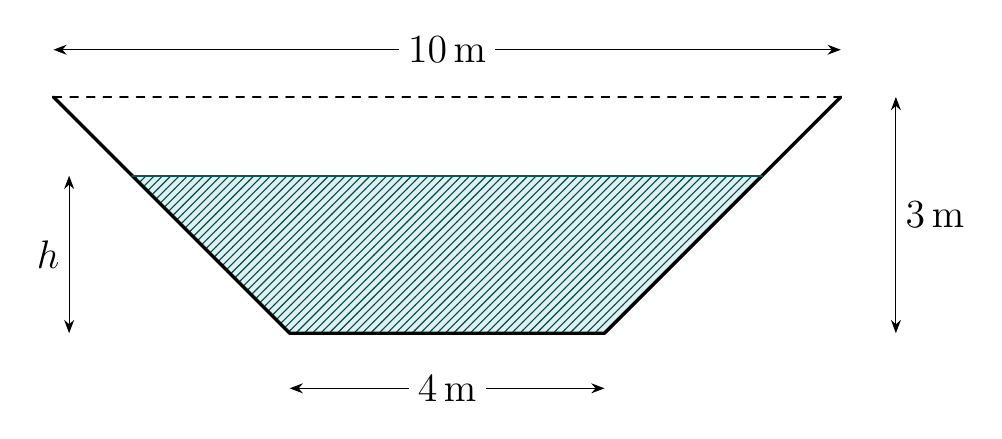
\begin{tikzpicture}[>=Stealth,line join=round,line cap=round,font=\Large]
\fill[teal!12] (-2,0)--(2,0)--(4,2)--(-4,2)--cycle;
\fill[pattern=north east lines,pattern color=teal!60!black] (-2,0)--(2,0)--(4,2)--(-4,2)--cycle;
\draw[very thick] (-5,3)--(-2,0)--(2,0)--(5,3);
\draw[dashed] (-5,3)--(5,3);
\draw[teal!70!black,thick] (-4,2)--(4,2);
\draw[<->] (-5,3.6)--(5,3.6) node[midway,fill=white] {$10\,\mathrm m$};
\draw[<->] (-2,-0.7)--(2,-0.7) node[midway,fill=white] {$4\,\mathrm m$};
\draw[<->] (5.7,0)--(5.7,3) node[midway,right] {$3\,\mathrm m$};
\draw[<->] (-4.8,0)--(-4.8,2) node[midway,left] {$h$};
\end{tikzpicture}}
\end{minipage}

\item \begin{minipage}[t]{0.55\linewidth}
Trong không gian $Oxyz$ (đơn vị: m), mặt đất là mặt phẳng $z=0$. Một bức tường kéo dài không giới hạn theo phương $Oy$ chiếm miền $0\leq x\leq2$, $0\leq z\leq3$. Một robot nhỏ bò từ $A(-4;1;0)$ đến $B(5;7;0)$ trên mặt đất và các mặt ngoài của tường. Robot có thể bám vào mặt đứng, đi qua nóc tường; không được xuyên tường hay rời bề mặt. Quãng đường ngắn nhất bằng bao nhiêu mét? Hình bên biểu diễn các mặt liên tiếp sau khi trải phẳng. \textit{(Làm tròn đến hàng phần mười.)}
\end{minipage}\hfill
\begin{minipage}[t]{0.42\linewidth}
\vspace{-0.4\baselineskip}\centering
\resizebox{\linewidth}{!}{%
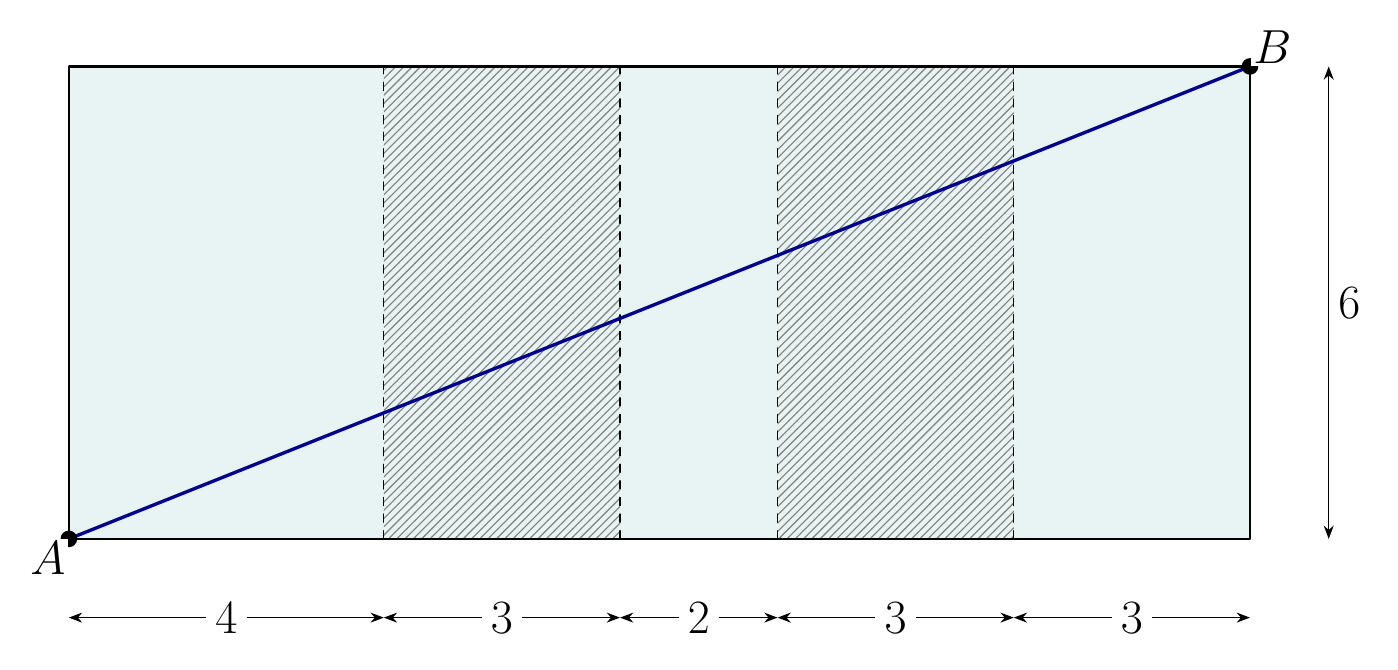
\begin{tikzpicture}[>=Stealth,line join=round,line cap=round,font=\LARGE]
\fill[teal!9] (0,0) rectangle (15,6);
\fill[pattern=north east lines,pattern color=gray] (4,0) rectangle (7,6);
\fill[pattern=north east lines,pattern color=gray] (9,0) rectangle (12,6);
\draw[thick] (0,0) rectangle (15,6);
\foreach \a in {4,7,9,12}{\draw[dashed] (\a,0)--(\a,6);}
\draw[blue!55!black,very thick] (0,0)--(15,6);
\fill (0,0) circle (3pt) node[below left,fill=white,inner sep=1pt] {$A$};
\fill (15,6) circle (3pt) node[above right,fill=white,inner sep=1pt] {$B$};
\foreach \a/\b/\c in {0/4/4,4/7/3,7/9/2,9/12/3,12/15/3}{
\draw[<->] (\a,-1)--(\b,-1) node[midway,fill=white] {$\c$};}
\draw[<->] (16,0)--(16,6) node[midway,right] {$6$};
\end{tikzpicture}}
\end{minipage}

\Needspace{7\baselineskip}
\item Trong không gian $Oxyz$ (đơn vị: m), hai thiết bị được đặt tại $A(2;1;3)$ và $B(5;1;0)$. Cần nối hai thiết bị bằng một sợi cáp gồm hai đoạn thẳng $AM$ và $MB$, với đầu nối $M$ nằm trên mặt phẳng $(P):2x-y+2z=0$. Bỏ qua độ dày và độ chùng của cáp. Chiều dài cáp ngắn nhất bằng bao nhiêu mét? \textit{(Làm tròn đến hàng phần mười.)}

\item \begin{minipage}[t]{0.55\linewidth}
Một mô hình kiến trúc cao $8$ m có mọi mặt cắt ngang vuông góc với trục thẳng đứng là hình vuông. Độ dài cạnh mặt cắt ở độ cao $h$ mét được mô tả bởi một hàm bậc hai $L(h)$ ($0\leq h\leq8$). Cạnh mặt đáy và mặt đỉnh đều dài $10$ m; mặt cắt hẹp nhất ở độ cao $4$ m có cạnh dài $6$ m. Thể tích mô hình bằng bao nhiêu mét khối? \textit{(Làm tròn đến hàng phần mười.)}
\end{minipage}\hfill
\begin{minipage}[t]{0.42\linewidth}
\vspace{-0.4\baselineskip}\centering
\resizebox{\linewidth}{!}{%
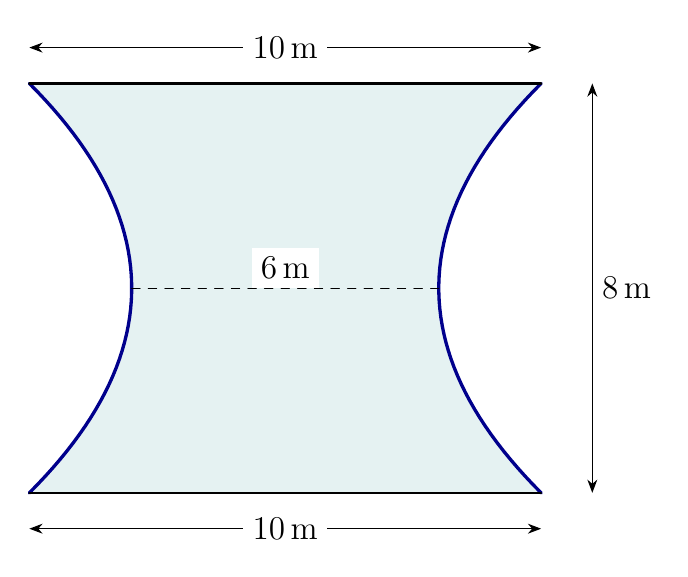
\begin{tikzpicture}[>=Stealth,line join=round,line cap=round,x=0.65cm,y=0.65cm,font=\large]
\fill[teal!10] plot[domain=0:8,samples=50] ({-3-(\x-4)^2/8},\x)--
plot[domain=8:0,samples=50] ({3+(\x-4)^2/8},\x)--cycle;
\draw[very thick,blue!55!black] plot[domain=0:8,samples=50] ({-3-(\x-4)^2/8},\x);
\draw[very thick,blue!55!black] plot[domain=0:8,samples=50] ({3+(\x-4)^2/8},\x);
\draw[thick] (-5,0)--(5,0) (-5,8)--(5,8);
\draw[dashed] (-3,4)--(3,4);
\draw[<->] (-5,-0.7)--(5,-0.7) node[midway,fill=white] {$10\,\mathrm m$};
\draw[<->] (-5,8.7)--(5,8.7) node[midway,fill=white] {$10\,\mathrm m$};
\node[above,fill=white] at (0,4) {$6\,\mathrm m$};
\draw[<->] (6,0)--(6,8) node[midway,right] {$8\,\mathrm m$};
\end{tikzpicture}}
\end{minipage}

\item Một máy công nghiệp được mua với giá $400$ triệu đồng. Khi máy đã hoạt động $t$ năm ($0\leq t\leq8$), tốc độ tạo doanh thu là $R'(t)=500-4t^2$ triệu đồng/năm và tốc độ phát sinh chi phí vận hành, bảo trì là $C'(t)=68+8t^2$ triệu đồng/năm. Ban đầu chưa có doanh thu và chi phí vận hành; sau khi ngừng sử dụng máy không có giá trị thanh lí. Chủ máy được chọn thời điểm ngừng sử dụng $T$ trong đoạn $[0;8]$. Lợi nhuận tích lũy lớn nhất sau khi trừ cả tiền mua máy bằng bao nhiêu triệu đồng?
\end{enumerate}
\begin{center}\textbf{--- HẾT ---}\end{center}

% BAT DAU DAP AN
\newpage
\begin{center}
{\Large\textbf{BẢNG ĐÁP ÁN TỔNG HỢP}}\\[4pt]
\textbf{ĐỀ SỐ 12 - MÃ ĐỀ 0012}
\end{center}
\medskip
\textbf{PHẦN I. TRẮC NGHIỆM NHIỀU PHƯƠNG ÁN}
\begin{center}\renewcommand{\arraystretch}{1.5}
\begin{tabular}{|*{12}{c|}}\hline
1 & 2 & 3 & 4 & 5 & 6 & 7 & 8 & 9 & 10 & 11 & 12\\\hline
B & D & A & C & D & B & A & C & A & D & B & C\\\hline
\end{tabular}\end{center}
\medskip
\textbf{PHẦN II. TRẮC NGHIỆM ĐÚNG SAI}
\begin{center}\renewcommand{\arraystretch}{1.5}
\begin{tabular}{|c|c|c|c|c|}\hline
Câu & a) & b) & c) & d)\\\hline
1 & S & Đ & Đ & S\\\hline
2 & Đ & S & S & Đ\\\hline
3 & Đ & Đ & S & S\\\hline
4 & Đ & S & Đ & Đ\\\hline
\end{tabular}\end{center}
\medskip
\textbf{PHẦN III. TRẮC NGHIỆM TRẢ LỜI NGẮN}
\begin{center}\renewcommand{\arraystretch}{1.5}
\begin{tabular}{|c|c|c|c|c|c|}\hline
1 & 2 & 3 & 4 & 5 & 6\\\hline
54,8 & 0,66 & 16,2 & 7,3 & 441,6 & 1328\\\hline
\end{tabular}\end{center}

\newpage
\begin{center}
{\Large\textbf{HƯỚNG DẪN GIẢI CHI TIẾT}}\\[4pt]
\textbf{ĐỀ SỐ 12 - MÃ ĐỀ 0012}
\end{center}
\section*{\large PHẦN I. TRẮC NGHIỆM NHIỀU PHƯƠNG ÁN}
\loigiai{Câu 1. Chọn B.}
Tập xác định là $\mathbb R\setminus\{1\}$. Ta có
\[
f(x)=x-1+\frac4{x-1},\qquad
f'(x)=1-\frac4{(x-1)^2}=\frac{(x-3)(x+1)}{(x-1)^2}.
\]
Vì mẫu số dương trên tập xác định, $f'(x)>0$ khi $x<-1$ hoặc $x>3$. Hàm số đồng biến trên $(-\infty;-1)$ và $(3;+\infty)$. Khoảng ở phương án B thỏa mãn.

\loigiai{Câu 2. Chọn D.}
Điều kiện $x>1$. Phương trình tương đương
\[
\log_2\big((x-1)(x+1)\big)=3
\ \Longleftrightarrow\ x^2-1=8
\ \Longleftrightarrow\ x=\pm3.
\]
Chỉ $x=3$ thỏa mãn điều kiện.

\loigiai{Câu 3. Chọn A.}
\[
\int_0^2(3x^2-2x+1)\,\mathrm dx
=\left[x^3-x^2+x\right]_0^2=8-4+2=6.
\]

\loigiai{Câu 4. Chọn C.}
Mặt phẳng vuông góc với đường thẳng nên nhận $\vec n=(1;2;-1)$ làm vectơ pháp tuyến. Phương trình qua $M$ là
\[
(x-2)+2(y+1)-(z-3)=0
\ \Longleftrightarrow\ x+2y-z+3=0.
\]

\loigiai{Câu 5. Chọn D.}
Có $\binom82=28$ cách chọn hai viên từ tám viên, trong đó $\binom52=10$ cách chọn hai viên đỏ. Xác suất cần tìm là
\[
P=\frac{\binom52}{\binom82}=\frac{10}{28}=\frac5{14}.
\]

\loigiai{Câu 6. Chọn B.}
Cỡ mẫu $n=30$, vị trí trung vị là $n/2=15$. Tần số tích lũy trước nhóm $[20;30)$ là $12$, nên nhóm này chứa trung vị. Với cận dưới $20$, độ rộng $10$, tần số $12$, ta được
\[
M_e=20+\frac{15-12}{12}\cdot10=22{,}5.
\]

\loigiai{Câu 7. Chọn A.}
Phương trình $\sin x=\tfrac12$ có nghiệm $x=\tfrac\pi6+2k\pi$ hoặc $x=\tfrac{5\pi}6+2k\pi$, $k\in\mathbb Z$. Trên $[0;2\pi)$ có đúng hai nghiệm $\tfrac\pi6$, $\tfrac{5\pi}6$.

\loigiai{Câu 8. Chọn C.}
Theo công thức số hạng tổng quát của cấp số nhân,
\[
u_5=u_1q^4=2\cdot3^4=162.
\]

\loigiai{Câu 9. Chọn A.}
Mặt cầu tiếp xúc với $(P)$ nên bán kính bằng khoảng cách từ tâm $I$ đến $(P)$:
\[
R=d(I,(P))=\frac{|2\cdot1-(-1)+2\cdot2+2|}{\sqrt{2^2+(-1)^2+2^2}}=\frac93=3.
\]

\loigiai{Câu 10. Chọn D.}
Đặt $u=x-2\ne0$, phương trình trở thành $u+3+4/u=m$, hay
\[
u^2-(m-3)u+4=0.
\]
Tích hai nghiệm bằng $4$, nên không có nghiệm $u=0$. Hai nghiệm thực phân biệt tồn tại khi
\[
\Delta=(m-3)^2-16>0
\ \Longleftrightarrow\ m<-1\ \text{hoặc}\ m>7.
\]
Trong $[-3;10]$, các giá trị nguyên phù hợp là $-3,-2,8,9,10$: có $5$ giá trị.

\loigiai{Câu 11. Chọn B.}
Do bố trí đối xứng, lực căng trong ba dây có cùng độ lớn $F$. Gọi $h$ là khoảng cách từ điểm treo đến mặt phẳng đèn. Với $r=0{,}6$ m và $L>r$,
\[
h=\sqrt{L^2-r^2},\qquad 3F\frac{h}{L}=90
\ \Longrightarrow\ F=\frac{30L}{\sqrt{L^2-0{,}36}}.
\]
Điều kiện an toàn $F\leq50$ tương đương
\[
\frac{\sqrt{L^2-0{,}36}}L\geq\frac35
\ \Longleftrightarrow\ 0{,}64L^2\geq0{,}36
\ \Longleftrightarrow\ L\geq0{,}75.
\]
Vậy mỗi dây ngắn nhất dài $0{,}75$ m; tại đó lực căng đúng bằng $50$ N.

\loigiai{Câu 12. Chọn C.}
Gọi $E$ là biến cố lấy được hai viên đỏ. Ta có
\[
P(E\mid A)=\frac{\binom42}{\binom62}=\frac25,
\qquad P(E\mid B)=\frac{\binom22}{\binom62}=\frac1{15}.
\]
Theo công thức Bayes,
\[
P(A\mid E)=\frac{\frac12\cdot\frac25}
{\frac12\cdot\frac25+\frac12\cdot\frac1{15}}=\frac67.
\]

\Needspace{10\baselineskip}
\section*{\large PHẦN II. TRẮC NGHIỆM ĐÚNG SAI}
\loigiai{Câu 1. a) Sai; b) Đúng; c) Đúng; d) Sai.}
Ta phân tích
\[
f(x)=x-2+\frac4{x-2},\qquad
f'(x)=1-\frac4{(x-2)^2}=\frac{x(x-4)}{(x-2)^2}.
\]
\begin{enumerate}[label=\alph*),leftmargin=*]
\item Tiệm cận đứng $x=2$, tiệm cận xiên $y=x-2$, nên $I(2;0)$. Khẳng định $y=x+2$ sai.
\item Đạo hàm đổi dấu từ dương sang âm qua $x=0$, từ âm sang dương qua $x=4$. Hai điểm cực trị là $(0;-4)$ và $(4;4)$, có khoảng cách
\[
\sqrt{(4-0)^2+(4+4)^2}=\sqrt{80}=4\sqrt5.
\]
\item Tại $x=3$, ta có $f(3)=5$, $f'(3)=-3$, nên tiếp tuyến là $y-5=-3(x-3)$, tức $y=-3x+14$. Giao với $x=2$ được $A(2;8)$; giao với $y=x-2$ được $B(4;2)$. Lấy $IA=8$ làm đáy, khoảng cách từ $B$ đến đường $IA$ là $2$, suy ra
\[
S_{IAB}=\frac12\cdot8\cdot2=8.
\]
\item Đặt $u=x-2$. Hai nghiệm cần thỏa mãn $0<u_1<u_2<6$ và là nghiệm của $u^2-mu+4=0$. Hai nghiệm dương phân biệt khi $m>4$. Với $u_2>2$, hàm $u+4/u$ đồng biến trên $(2;+\infty)$, nên
\[
u_2<6\ \Longleftrightarrow\ m<6+\frac46=\frac{20}3.
\]
Vậy $4<m<20/3$, chỉ có $m=5,6$, tức $2$ giá trị nguyên.
\end{enumerate}

\loigiai{Câu 2. a) Đúng; b) Sai; c) Sai; d) Đúng.}
Gọi $D$ là biến cố linh kiện thực sự lỗi, $E$ là biến cố cả hai lần kiểm tra đều báo lỗi. Từ giả thiết độc lập có điều kiện,
\[
P(E\mid D)=0{,}9^2=0{,}81,\qquad
P(E\mid\overline D)=0{,}1^2=0{,}01.
\]
\begin{enumerate}[label=\alph*),leftmargin=*]
\item Theo công thức xác suất toàn phần,
\[
P(D)=0{,}4\cdot0{,}02+0{,}6\cdot0{,}05=0{,}038.
\]
\item Theo Bayes,
\[
P(A\mid D)=\frac{0{,}4\cdot0{,}02}{0{,}038}=\frac4{19},
\]
không phải $6/19$.
\item Xác suất hai lần đều báo lỗi là
\[
P(E)=0{,}038\cdot0{,}81+0{,}962\cdot0{,}01
=0{,}03078+0{,}00962=0{,}0404,
\]
không phải $0{,}0344$. Không được tính bằng $P(\text{một lần báo lỗi})^2$ vì hai lần chỉ độc lập khi đã biết trạng thái linh kiện.
\item Xác suất cần xét là
\[
P(D\mid E)=\frac{0{,}038\cdot0{,}81}{0{,}0404}
=\frac{1539}{2020}\approx0{,}761881>0{,}75.
\]
\end{enumerate}

\loigiai{Câu 3. a) Đúng; b) Đúng; c) Sai; d) Sai.}
Khoảng cách bình phương từ drone đến radar là
\[
OM^2=(-7+2t)^2+(-10+2t)^2+(-2+t)^2
=9t^2-72t+153=9(t-4)^2+9.
\]
\begin{enumerate}[label=\alph*),leftmargin=*]
\item Khi $t=0$, $OA=\sqrt{153}=3\sqrt{17}$ km.
\item Giá trị nhỏ nhất của $OM^2$ là $9$, đạt tại $t=4\geq0$. Vị trí gần nhất là $H(1;-2;2)$, khoảng cách nhỏ nhất $OH=3$ km.
\item Radar phát hiện drone khi
\[
9(t-4)^2+9\leq25
\ \Longleftrightarrow\ \frac83\leq t\leq\frac{16}3.
\]
Khoảng thời gian phát hiện dài $16/3-8/3=8/3$ phút, không phải $3$ phút.
\item Nếu bán kính mới là $R\geq3$, đặt $a=\sqrt{R^2-9}/3$. Trên toàn đường bay, điều kiện phát hiện là $4-a\leq t\leq4+a$. Với $a\leq4$, cả hai thời điểm đều không âm, thời gian phát hiện là $2a$. Để đạt ít nhất $4$ phút cần $a\geq2$, tức $R\geq3\sqrt5\approx6{,}71$ km. Nếu $a>4$, drone đã trong vùng phát hiện ở $t=0$ và thời gian còn phát hiện là $4+a>8$ phút, nên vẫn thỏa mãn. Bán kính $6$ km chỉ cho thời gian $2\sqrt3\approx3{,}46$ phút, chưa đủ.
\end{enumerate}

\loigiai{Câu 4. a) Đúng; b) Sai; c) Đúng; d) Đúng.}
Các giá trị đại diện của năm nhóm lần lượt là $49,51,53,55,57$ gam; cỡ mẫu $n=50$.
\begin{enumerate}[label=\alph*),leftmargin=*]
\item Trung bình ghép nhóm là
\[
\overline x=\frac{5\cdot49+10\cdot51+20\cdot53+10\cdot55+5\cdot57}{50}=53.
\]
\item Phương sai là
\[
s_X^2=\frac{5\cdot(-4)^2+10\cdot(-2)^2+20\cdot0^2+10\cdot2^2+5\cdot4^2}{50}
=\frac{240}{50}=4{,}8.
\]
Khẳng định $4{,}6$ sai.
\item Vị trí hai tứ phân vị là $12{,}5$ và $37{,}5$. Nhóm chứa $Q_1$ là $[50;52)$, nhóm chứa $Q_3$ là $[54;56)$:
\[
Q_1=50+\frac{12{,}5-5}{10}\cdot2=51{,}5,\qquad
Q_3=54+\frac{37{,}5-35}{10}\cdot2=54{,}5.
\]
Do đó $\Delta_Q=Q_3-Q_1=3$ gam.
\item Với $Y=0{,}5X+26{,}5$, các nhóm và giá trị đại diện cùng được biến đổi tuyến tính. Ta có
\[
\overline y=0{,}5\overline x+26{,}5=53,\qquad
s_Y^2=0{,}5^2s_X^2=1{,}2,\qquad s_Y=0{,}5s_X.
\]
Vì vậy trung bình không đổi và độ lệch chuẩn còn một nửa.
\end{enumerate}

\Needspace{10\baselineskip}
\section*{\large PHẦN III. TRẮC NGHIỆM TRẢ LỜI NGẮN}
\loigiai{Câu 1. Đáp số: 54,8.}
Từ $n(e^2-1)=A+40\ln(e^2)=A+80=200$, suy ra $A=120$.
Lãi trên mỗi chiếc trước chi phí quảng cáo là $800-500=300$ nghìn đồng, tức $0{,}3$ triệu đồng. Hàm lợi nhuận, đơn vị triệu đồng, là
\[
P(x)=0{,}3\big(120+40\ln(1+x)\big)-x
=36+12\ln(1+x)-x,\qquad x\geq0.
\]
Đạo hàm $P'(x)=12/(1+x)-1=(11-x)/(1+x)$ dương trên $[0;11)$ và âm trên $(11;+\infty)$. Do đó lợi nhuận đạt lớn nhất tại $x=11$:
\[
P_{\max}=36+12\ln12-11=25+12\ln12\approx54{,}8188798.
\]
Làm tròn đến hàng phần mười: $54{,}8$ triệu đồng.

\loigiai{Câu 2. Đáp số: 0,66.}
Gọi $h$ là độ cao mực nước tính từ đáy. Do thành bể thẳng, chiều dài mặt cắt ngang biến thiên tuyến tính:
\[
\ell(h)=4+\frac{10-4}{3}h=4+2h.
\]
Diện tích mặt cắt ngang $S(h)=6(4+2h)$, nên thể tích nước đến độ cao $h$ là
\[
V(h)=\int_0^h6(4+2u)\,\mathrm du=24h+6h^2.
\]
Khi $h=2$, thể tích $V=72$ m$^3$. Lượng nước đã bơm đến thời điểm $t$ là
\[
\int_0^t(6u+12)\,\mathrm du=3t^2+12t.
\]
Giải $3t^2+12t=72$ với $t\geq0$ được $t=2\sqrt7-2$. Khi đó $q(t)=12\sqrt7$ m$^3$/phút. Vi phân theo thời gian cho $\mathrm dV/\mathrm dt=S(h)\,\mathrm dh/\mathrm dt$, nên
\[
\left.\frac{\mathrm dh}{\mathrm dt}\right|_{h=2}
=\frac{12\sqrt7}{6(4+2\cdot2)}=\frac{\sqrt7}{4}
\approx0{,}6614378.
\]
Làm tròn: $0{,}66$ m/phút. Mực nước $2$ m nhỏ hơn chiều sâu $3$ m nên bể chưa tràn.

\loigiai{Câu 3. Đáp số: 16,2.}
Do tường kéo dài vô hạn theo phương $Oy$, mọi đường đi nối hai phía phải lần lượt qua mặt đất bên trái, mặt đứng bên trái, nóc tường, mặt đứng bên phải và mặt đất bên phải. Trải phẳng năm phần này, tổng độ rộng theo phương vượt tường là
\[
4+3+2+3+(5-2)=15\ \text{m}.
\]
Độ chênh theo phương $Oy$ là $7-1=6$ m. Việc trải phẳng giữ nguyên độ dài đường đi. Mọi đường nối hai điểm trên hình trải phẳng dài ít nhất bằng đoạn thẳng nối chúng. Đoạn thẳng đó lần lượt cắt các nếp gấp và khi gấp lại tạo được một đường đi hợp lệ trên đủ năm mặt, nên cận dưới đạt được:
\[
d_{\min}=\sqrt{15^2+6^2}=\sqrt{261}=3\sqrt{29}\approx16{,}1554944.
\]
Làm tròn đến hàng phần mười: $16{,}2$ m.

\loigiai{Câu 4. Đáp số: 7,3.}
Mặt phẳng $(P)$ có vectơ pháp tuyến $\vec n=(2;-1;2)$ với $\|\vec n\|^2=9$. Giá trị $2x-y+2z$ tại $A$ và $B$ đều bằng $9$, nên hai điểm nằm cùng phía đối với $(P)$.
Phản xạ $A$ qua $(P)$ được
\[
A'=A-2\frac{\vec n\cdot\overrightarrow{OA}}{\|\vec n\|^2}\vec n
=(2;1;3)-2(2;-1;2)=(-2;3;-1).
\]
Với mọi $M\in(P)$, $AM=A'M$, nên bất đẳng thức tam giác cho
\[
AM+MB=A'M+MB\geq A'B.
\]
Hai điểm $A'$ và $B$ ở hai phía của $(P)$, vì vậy đoạn $A'B$ cắt $(P)$ tại một điểm $M$ và dấu bằng đạt được. Cụ thể, do khoảng cách có hướng của hai điểm bằng nhau về độ lớn, $M$ là trung điểm $A'B$, tức $M(3/2;2;-1/2)$. Suy ra
\[
d_{\min}=A'B=\sqrt{(5+2)^2+(1-3)^2+(0+1)^2}
=\sqrt{54}=3\sqrt6\approx7{,}3484692.
\]
Làm tròn đến hàng phần mười: $7{,}3$ m.

\loigiai{Câu 5. Đáp số: 441,6.}
Hàm bậc hai $L(h)$ đạt nhỏ nhất bằng $6$ tại $h=4$, nên $L(h)=a(h-4)^2+6$ với $a>0$. Điều kiện $L(0)=10$ cho $16a+6=10$, suy ra $a=1/4$. Công thức này cũng thỏa $L(8)=10$.
Diện tích mặt cắt ngang là $S(h)=L(h)^2$, không phải $L(h)$. Thể tích là
\[
V=\int_0^8\left(6+\frac{(h-4)^2}{4}\right)^2\,\mathrm dh.
\]
Đặt $u=h-4$, tận dụng tính chẵn:
\[
V=2\int_0^4\left(36+3u^2+\frac{u^4}{16}\right)\,\mathrm du
=2\left[36u+u^3+\frac{u^5}{80}\right]_0^4
=\frac{2208}{5}=441{,}6\ \mathrm m^3.
\]

\loigiai{Câu 6. Đáp số: 1328.}
Lợi nhuận tích lũy sau $T$ năm, trừ cả tiền mua máy, là
\[
P(T)=\int_0^T\big[(500-4t^2)-(68+8t^2)\big]\,\mathrm dt-400
=432T-4T^3-400,\quad 0\leq T\leq8.
\]
Đạo hàm $P'(T)=432-12T^2=12(36-T^2)$ dương khi $0\leq T<6$, bằng $0$ khi $T=6$ và âm khi $6<T\leq8$. Do đó $P$ đạt giá trị lớn nhất tại $T=6$:
\[
P_{\max}=432\cdot6-4\cdot6^3-400
=2592-864-400=1328\ \text{triệu đồng}.
\]
\begin{center}\textbf{--- HẾT LỜI GIẢI ---}\end{center}
\end{document}
